\documentclass[paper=a4paper,fontsize=10pt,jafontscale=0.925,twocolumn]{jlreq}
\usepackage{luatexja}
\usepackage{lab-handout}

% ここから上は変更しない

\title{審査資料テンプレート} % 自身の卒業研究/修士論文の予定表題に変更

%以下は適切な所属を1つ選択
%\affiliation{人間システム工学科 井村研究室} % 卒業研究(人間システム工学科)
\affiliation{知能・機械工学課程 井村研究室} % 卒業研究(知能・機械工学課程)
%\affiliation{人間システム工学専攻 井村研究室} % 修士論文

\studentnumber{37019999} % 8桁の学籍番号
\author{井村 誠孝} % 姓名間の空白は半角で

\graphicspath{{./figure/}} % 画像を置いておくフォルダ名

\begin{document}

\maketitle

\section{はじめに}

本テンプレートは,卒業研究および修士論文の審査資料を作成する際に
使用するものである.

\section{節見出し}

最初の節の見出しと最後の節の見出しは対応させることが一般的である.
表\ref{table:section_name}に対応の例を示す.
ただし,\textgt{中間審査の場合は,研究の途上であるため,
最初の節「はじめに」に対して最後の節「まとめと今後の課題」で結ぶ.}

「提案手法」「実験」といった汎用的な節見出しよりは,
「映像提示手法」「画質評価実験」といった具体性のある節見出しがよい.
また節見出し(section)と小節見出し(subsection)に同一の文言を使うことはしない.
節は小節を複数含むようにする.
節内に小節が1個しか無い場合は,小節は不要なはずである.

\section{図・表}

\subsection{図表の選択}

審査資料の紙面は限られているため,図表の選択は迷うところであるが,
文章だけの資料は魅力に欠けるため,最低1枚は入れるように心がける.

選択の基準として,審査の目的は研究の遂行度合いを確認するためであるから,
研究を遂行していることの証明となる図表がよい.
自分の作成したシステムの写真やスクリーンショットは,文字では伝えられない情報を伝達できるため有用である.
次に,システム構成や処理フロー(図\ref{fig:flow})の図がよい.提案手法や実験内容をわかりやすく伝える効果がある.

\subsection{図表の配置}

図表の配置位置には二つの流儀がある.
\begin{enumerate}
 \item 集約型: 紙面の上端あるいは下端に集約する.
 \item 文中型: 本文中で参照した箇所を含む段落の直後に配置する.
\end{enumerate}
\textgt{上端集約型が文章と図表が分離されていてすっきりしているため,
原則として上端集約型で配置する.}
figureやtable環境のオプションとして\verb|tp|を指定する.

%上端に集約する際は,
本文が始まる前に図表が入ることは避ける.
二段組の場合,1ページ目の左上には入れない.右上はよい.

%文中型の場合は,段落と段落の間に入れるようにする.
%文が図表で分断されるのは不可である.

図表は本文中で必ず参照する.
%集約型の場合,
図表は参照箇所と同じページ(二段組の場合には同じ段)か,参照箇所より後のページ(二段組の場合には後の段)に置く.
%参照箇所よりも前のページ(二段組の場合には前の段)に,図表が配置されるのは不可である.
適切な箇所に\LaTeX{}が配置してくれるように,ソース中の図表配置位置を適宜移動させる.

\subsection{キャプション}

図表には適切なキャプション(説明)を付ける.
図のキャプションは図の下,表のキャプションは表の上に配置する.

\section{参考文献}

参考文献は,学術的な内容のものを必ず1件は挙げる.
読み物やマニュアル類,URLだけは不可である.

参考文献はBibTeXを用いることを推奨する.
不要な情報が表記されてしまう場合は,BibTeXのエントリー名を変更して非表示にする.
例: \verb|month|を\verb|OPTmonth|など.

参考文献は本文中で参照している文献のみを登場順に並べて掲載する.
BibTeXを用いれば自動的に行われる.
参照の例\cite{Gao2018}.
詳しくは\cite{Okumura2017}を見よ.

\begin{table}[tp]
 \centering
 \caption{最初の節の見出しと最後の節の見出しの対応}
 \begin{tabular}{c|c} \hline
  最初の節の見出し & 最後の節の見出し \\ \hline
  はじめに & おわりに \\
  緒言 & 結言 \\
  序論 & 結論 \\ \hline
 \end{tabular}
 \label{table:section_name}
\end{table}

\begin{figure}[tp]
 \centering
 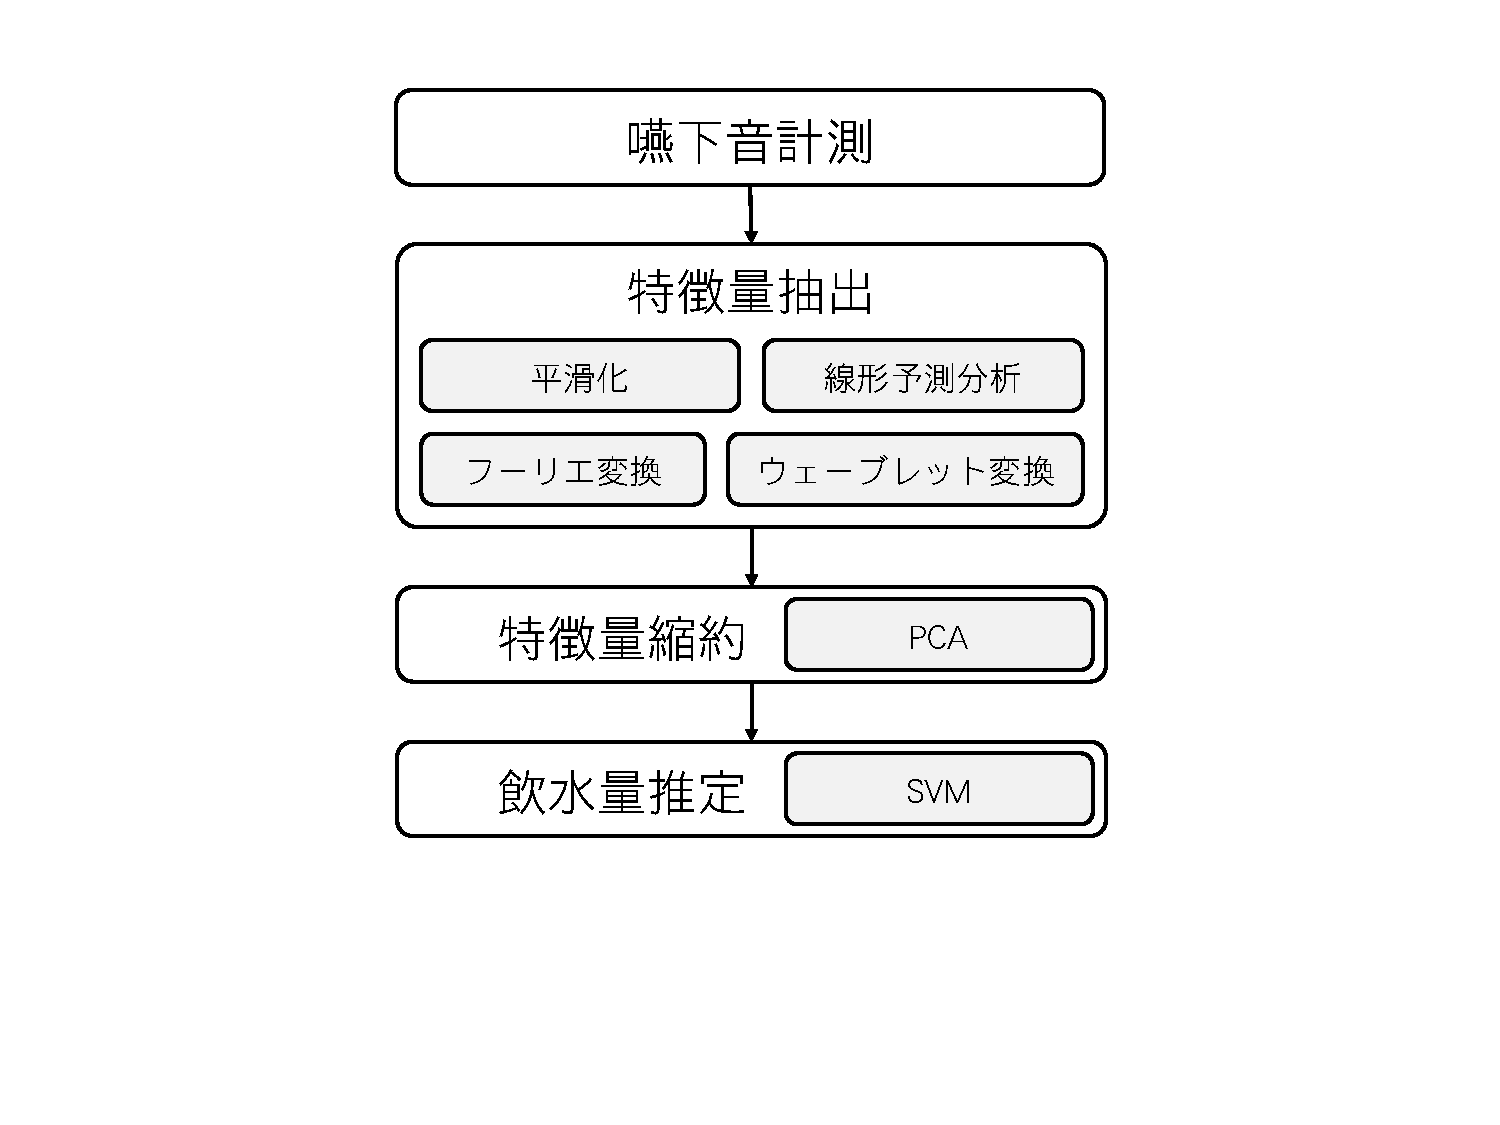
\includegraphics[width=0.22\textwidth]{flowchart.pdf}
 \caption{処理の流れ}
 \label{fig:flow}
\end{figure}

\section{その他}

文末は「だ,である」で統一する.

表記にぶれがないようにする.
%特に,研究に特有の用語の統一に気を配る.

句読点は「,.」か「、。」のいずれでも可だが,\textgt{全角の「,.」の使用を推奨する.}
半角の「,」あるいは「.」と半角の空白を並べると空白が一定せずバランスが悪いため,和文では使用しない.

原則として,提案手法までは現在形,試作システムの作成や実験以降に行った内容については過去形で記述する.

\section{まとめと今後の課題} % 中間審査の場合
%\section{おわりに} % 最終審査の場合

まとめは本審査資料のまとめであり,現時点での研究の総括でもあるはずである.
おおむね,
「本研究では$\cdots$を目的として$\cdots$を提案した.」
「本稿では$\cdots$について述べた.」
「実験により,$\cdots$であることが示された.」
といった内容になる.
紙面が不足する場合,最初の「本研究では$\cdots$」は省略してもよい.

今後の課題は,この研究が期限までに完了する目処が立っていることを示すために書く.
したがって,次に行う具体的な作業だけを述べるのではなく,研究を終えるまでに行う予定のことを整理して記述する.

\bibliographystyle{plain}
\bibliography{reference}

\end{document}